
% Last updated: (probably) April 1, 2022
\documentclass[11pt, oneside,margin=1in]{article}

\def\jtitle{Modular forms}
\def\jlecturer{Dr. Richard Borcherds}
\def\jterm{}
\def\jauthor{Jack DeSerrano}
\usepackage[course]{jack}


\title{Modular forms}
\author{Jack DeSerrano}

\begin{document}
\ifams
    \topskip0pt
    \vspace*{\fill}
\fi
\maketitle
These notes are based on Richard Borcherds's YouTube series on modular forms\footnote{See \url{https://www.youtube.com/playlist?list=PL8yHsr3EFj51HisRtNyzHX-Xyg6I3Wl2F}.}.
\ifams
	\vspace*{\fill}
\fi
\vfill
\begin{center}
	``There are five fundamental operations of arithmetic: addition, subtraction, multiplication, division, and modular forms.'' --- Martin Eichler
\end{center}
{\vfill}
\newpage
\section{Introduction}
\begin{definition}[Modular form]\label{}\text{}
Let 
\begin{align*}
	\mat{a&b\\c&d} \in \SL_{2}(\Z).
\end{align*}
A \defn{modular form}\index{modular form} is a function $f$ on the upper-half plane satisfying
\begin{align*}
	f\left( \frac{a\tau + b}{c\tau + d} \right) = (c\tau + d) ^k f(\tau).
\end{align*}
\end{definition}
\begin{example}[Modular function]\label{}\text{}
A function satisfying this definition when $k=0$ is a \defn{modular function}\index{modular function}. Now, consider this convoluted function:
\begin{align*}
	j(\tau) :=  \frac{\left(1 + 240 \sum_{n>0}^{} \sigma_3(n)q^n \right)^3}{q \prod_{n>0} (1-q^n)^{24}},\ q= \exp(2\pi i \tau)
\end{align*}
where
\begin{align*}
	\sigma_3(n) :=  \sum_{d\, \mid\,  n}^{} d^3.
\end{align*}
This turns out to be the simplest non-constant modular function.
\end{example}

Where does $j$ show up?

\begin{example}[Finite groups]\label{}\text{}
The monster group is the largest sporadic simple group: it has approximately $10^{54}$ elements and lives in $196883$ dimensions. The modular function $j$ has a Laurent series expansion:
\begin{align*}
	j(\tau) = q ^{-1} + 744 + 196884q + 21493760q^2 + \cdots.
\end{align*}
McKay discovered the mysterious fact that the coefficient of $q$ is $1$ more than $196883$, and it turned out that the other coefficients relate similarly to the monster group. This is a typical example of a striking relationship between the theory of modular forms and some apparently unrelated field in mathematics. 
\end{example}

Here's another interesting property of $j$:
\begin{align*}
	j\left( \frac{1+\sqrt{-163} }{2} \right) = -262537412640768000\in \Z.
\end{align*}
This relates to the well-known fact that 
\begin{align*}
	\exp(\pi \sqrt{163} ) = 262537412640768743.99999999999925\cdots
\end{align*}
is very close to an integer. A brief look at the $q$-expansion of $j$ corroborates this. (For this $\tau$, $q=-\exp(-\pi\sqrt{163} )$.)

What else?

\begin{example}[Sphere packing]\label{}\text{}
Kepler\footnote{``On the six-cornered snowflake,'' 1611.} conjectured that no arrangement of equally sized spheres filling space has density greater than $\pi/\sqrt{18}$. Hales\footnote{``A proof of the Kepler conjecture.''} proved this in 1998, and his method was considerably complicated. 

While the next dimensions after $3$ are mostly unknown, optimal sphere packings in dimensions $8$ and $24$ are known. Take all points $(n_1,\hdots, n_8)$ with $\sum_{i}^{} n_i$ even and all $n_i\in \Z$ or all $n_i\in \Z + 1/2$. These are the centres of the spheres. This packing had been known for a while, but Maryna Viazovska used modular forms---a process that involved miraculous coincidences and cancellations---to prove that it was optimal\footnote{See \url{https://arxiv.org/abs/1603.04246}.}. Her method only works in $8$ and $24$ dimensions.

The dimensions $8$ and $24$ appear frequently in the theory of modular forms, but no one really knows why. There happen to be
\begin{align*}
	240\sigma_3(n)
\end{align*}
spheres at a distance $\sqrt{2n} $ from the origin in this $8$-dimensional packing. This showed up in the definition of $j$.
\end{example}


What else? 
\begin{example}[Fermat's last theorem]\label{}\text{}
Frey related Fermat's last theorem to the elliptic curve $y^2 = x(x-a^n) (x+b^n)$. Serre and Ribet related this elliptic curve to a modular form---showed that the Taniyama--Shimura--Weil conjecture implies Fermat's last theorem. Wiles, in essence, showed that any curve of the form above has an associated modular form: Consider
\begin{align*}
	y^2 - y = x^3-x^2.
\end{align*}
The number of solutions to this mod $p$ is $p-c_p$ where $c_p$ is the coefficient of $q^n$ in 
\begin{align*}
	q\prod_{n>0} (1-q^n)^2 (1-q^{11n})^2.
\end{align*}
This turns out to be a modular form. Frey, Serre, and Ribet proved that if there is a modular form associated to the Frey curve, then a contradiction arises. 
\end{example}

More!

\begin{example}[Langlands program]\label{}\text{}
The Langlands program, which is tightly related to Wiles's proof of Fermat's last theorem, says that there is a correspondence between Galois representations
\begin{align*}
	\rho : \Gal(\ol \Q/\Q)  \longrightarrow \GL_{n}(\R)
\end{align*}
and modular forms---more generally, automorphic forms. Wiles proved a tiny part of the harder direction of this. Another special case is $n=1$, which turns out to be class field theory.
\end{example}

\begin{example}[Riemann zeta function]\label{}\text{}
Recall:
\begin{align*}
	\zeta(s) :=  \sum_{k}^{} 1/k^s.
\end{align*}
Well, Riemann pointed out that
\begin{align*}
	\pi^{-s/2} \Gamma(s/2) \zeta (s) =  \frac{1}{2}\int_{0}^{\infty} \vartheta(i\tau) \tau^{s/2-1}  \, d\tau 
\end{align*}
where 
\begin{align*}
	\vartheta(i\tau) =  \sum_{n}^{} \exp(n^2\pi i \tau). 
\end{align*}
(This integral does not converge for any $s$.) But, $\vartheta$ is a modular form. Riemann used this to show the functional equation for the zeta function: that is, if 
 \begin{align*}
	\zeta^*(s) := \pi^{-s/2} \Gamma(s/2) \zeta (s),
\end{align*}
then $\zeta^* (s) = \zeta^* (1-s)$.
\end{example}

\begin{example}[Jacobi triple product]\label{}\text{}
Jacobi:
\begin{align*}
	&1 - q(z+z^{-1}) + q^4(z^2 + z^{-2}) + q^9  (z^3 + z^{-3}) + \cdots \\ =\,\, & (1-qz) (1-qz^{-1})(1-q^2) (1-q^3z) (1-q^3z^{-1}) (1-q^4)\cdots.
\end{align*}
Both sides of this are a modular form (provided $z$ is a root of unity). One special case of this is
\begin{align*}
	1 + 2q + 2q^4 + 2q^9 + \cdots = (1+q)^2 (1-q^2) (1+q^3)^2 (1-q^4)\cdots,
\end{align*}
a modular form.
\end{example}
	
We connected the numerator of the definition of $j$ to sphere packing, so what about the denominator? Let's look at it:
\begin{align*}
	q \prod_{n>0} (1-q^n)^{24} = q - 24q^2 + 252q^3 - 1452q^4 + 4830q^5 - 6048q^6 + \cdots = \sum_{n}^{} q^n\tau(n).
\end{align*}
Ramanujan noticed that 
\begin{align*}
	\tau(mn) = \tau (m)\tau (n)
\end{align*}
when $m$ and $n$ are coprime. Replace $24$ with almost any other number, and nothing like this happens (the magic of $24$). This is obtained using Hecke operators. 
\begin{problem}
	Find all modular forms of level $1$.
\end{problem}


\section{Eisenstein series}
Recall the definition of a modular form. In the ``$k=0$ case''---modular functions---$f$ is invariant under the action of $\SL_{2}(\mathbf{Z})$ on the upper-half plane:
\begin{align*}
	\mat{a&b\\c&d} (\tau) =  \frac{a\tau + b}{c\tau + d}.
\end{align*}

These functions are functions of elliptic curves:
\begin{align*}
	f : \big\{\ \textrm{elliptic curves $E$}\ \big\} \longrightarrow \C.
\end{align*}
(Such functions are sometimes called \defn{moduli functions}\index{moduli function}.) Suppose $g$ is such a function. For periods $\omega_1$ and $\omega_2$ of the curve, we require
\begin{align*}
	g(\omega_1,\omega_2) = g(\lambda\omega_1,\lambda\omega_2),\ \lambda\in \C^*.
\end{align*}
For 
\begin{align*}
A=	\mat{a&b\\c&d} \in \GL_{2}(\Z),\ \det A = \pm 1, 
\end{align*}
we also require
\begin{align}\label{thing}
	g(a\omega_1+b\omega_2, c\omega_1+d\omega_2) = g(\omega_1,\omega_2).
\end{align}
(That is, $g$ is invariant under a change of basis of the lattice.) For notation,
 \begin{align*}
	f(\tau) := g (1,\tau).
\end{align*}
Therefore, $g(\omega_1,\omega_2) = f(\omega_2/\omega_1)$. Rewriting \cref{thing} in terms of $f$, we get the desired invariance:
\begin{align*}
	f\left( \frac{a\tau + b}{c\tau +d} \right) = f(\tau).
\end{align*}
Here, $\tau$ must be non-real, but it is convenient to assert that $\Im(\tau) > 0$ (applying $\tau\longmapsto -\tau$ when that's necessary). That is, we restrict our concerns to the case
\begin{align*}
	\det A = +1.
\end{align*}

\begin{problem}
	Find (holomorphic) functions $f$ that satisfy the invariance
	\begin{align*}
		f\left( \frac{a\tau + b}{c\tau +d} \right) = f(\tau).
	\end{align*}
\end{problem}

This is difficult, so let's consider something easier.

\begin{problem}
	Find modular forms.
\end{problem}

Instead of finding an invariant function $f(\tau)$, we might find an invariant one-form:
 \begin{align*}
	f(\tau)\, d\tau = f \left( \frac{a\tau + b}{c\tau + d} \right) \frac{d\tau}{(c\tau+d)^2}.
\end{align*}
That is,
\begin{align*}
f\left( \frac{a\tau+b}{c\tau +d} \right) = (c\tau+d) ^2 f(\tau).	
\end{align*}
A function satisfying this functional equation is called a modular form of weight $2$. (Notice that the \defn{weight}\index{weight} of a modular form is the exponent on $c\tau + d$.) We don't have to restrict our discussion to one-forms: $f(\tau) \, (d\tau)^{k/2}$ is invariant if and only if
\begin{align*}
	f\left( \frac{a\tau+b}{c\tau +d} \right) = (c\tau + d) ^k  f(\tau).
\end{align*}
Then, $f$ is a modular form of weight $k$. You can think of this $f(\tau)\,  (d\tau)^{k/2}$ as a formal symbol that transforms as above or as a section of a line bundle.

Suppose $f_1(\tau)\,  (d\tau)^{k/2}$ and $f_2(\tau)\,  (d\tau)^{k/2}$ are invariant. Then
\begin{align*}
	\frac{f_1(\tau) \,  (d\tau)^ {k/2}}{f_2(\tau)\,  (d\tau)^{k/2}} = \frac{f_1(\tau)}{f_2(\tau)}
\end{align*}
is invariant. This is a modular function! 

How do we get modular forms, though? Let $g$ be a homogeneous function of a lattice: so
\begin{align*}
	g (\lambda\omega_1,\lambda\omega_2) = \lambda^{-k} g(\omega_1,\omega_2)
\end{align*}
and, still,
\begin{align*}
	g(a\omega_1+b\omega_2,c\omega_1+d\omega_2) = g(\omega_1,\omega_2).
\end{align*}
Defining $f$ as before, we get the desired functional equation:
\begin{align*}
	f\left( \frac{a\tau+b}{c\tau+d} \right) = (c\tau+d) ^k f(\tau).
\end{align*}

Now, we have three ways to view modular forms of weight $k$:
\begin{enumerate}
	\item Functions $f$ satisfying
		\begin{align*}
			f\left( \frac{a\tau+b}{c\tau+d} \right) = (c\tau+d) ^k f(\tau) ;
		\end{align*}
	\item Invariant forms $f(\tau) \,  (d\tau) ^{k/2}$;
	\item Homogeneous functions of lattices ``of weight $k$.''
\end{enumerate}

\begin{example}[Weierstrass elliptic function]\label{}\text{}
Recall:
\begin{align*}
	\wp(z,\omega_1,\omega_2) := \frac{1}{z^2} + \sum_{\substack{m,n\in \Z\\(m,n)\ne (0,0)}}^{}\left( \frac{1}{(z- m\omega_1 - n\omega_2)^2} - \frac{1}{(m\omega_1 + n\omega_2)^2}\right).
\end{align*}
Notice that
\begin{align*}
	\wp (\lambda z,\lambda \omega_1,\lambda\omega_2) = \lambda^{-2} \wp(z,\omega_1,\omega_2).
\end{align*}
Let's look at its Laurent series in $z$:
\begin{align*}
	\wp(z) = z^{-2} + a_2z^2 + a_4z^4 + \cdots.
\end{align*}
The coefficients $a_2$, $a_4$, etc. are functions of $\omega_1$ and $\omega_2$: the homogeneity relation gives
\begin{align*}
	(\lambda z)^{-2} +  a_2(\lambda\omega_1,\lambda\omega_2) (\lambda z)^2 + \cdots = \lambda^{-2}  (z^{-2} + a_2(\omega_1,\omega_2)z^2+\cdots).
\end{align*}
However,
\begin{align*}
	a_2(\lambda\omega_1,\lambda\omega_2) &= \lambda^{-4} a_2(\omega_1,\omega_2);\\
	a_4(\lambda \omega_1,\lambda\omega_2) &= \lambda^{-6} a_4(\omega_1,\omega_2);
\end{align*}
etc. These coefficients are almost modular forms:
\begin{align*}
	\alpha_k (\tau) := a_{k-2}(1,\tau)
\end{align*}
is a modular form of weight $k$. 

Now,
\begin{align*}
	\frac{1}{(z-m\omega_1-n\omega_2)^2} = \frac{1}{(m\omega_1+n\omega_2)^2} + \frac{2z}{(m\omega_1+n\omega_2)^3} + \frac{3z}{(m\omega_1+n\omega_2)^4} + \cdots.
\end{align*}
So, the coefficient of $z^{k-2}$ in $\wp(z,\omega_1,\omega_2)$ is
\begin{align*}
	\textrm{constant} \times \sum_{\substack{m,n\in \Z\\(m,n)\ne (0,0)}}^{} \frac{1}{(m\omega_1+n\omega_2) ^k}.
\end{align*}
Fix $\omega_1=1$, and we get
\begin{align*}
	\sum_{\substack{m,n\in \Z\\(m,n)\ne (0,0)}}^{} \frac{1}{(m+n\tau)^k}.
\end{align*}
This is an \defn{Eisenstein series}\index{Eisenstein series}. We only consider even $k$ (otherwise the series is $0$), and we take $k\ge 4$ since this is not absolutely convergent when $k=2$ (though that case is interesting).

This series is invariant under $\tau \longmapsto \tau+1$: under the matrix
 \begin{align*}
	 \mat{1&1\\0&1}.
\end{align*}
We can consider its $q$-expansion:
\begin{align*}
	c_0 + c_1q + c_2q^2 + \cdots,\ q=\exp(2\pi i\tau).
\end{align*}
\begin{problem}
	Compute these Fourier coefficients $c_n$.
\end{problem}
\end{example}

Recall that we can also see modular forms as invariant forms $f(\tau)\,  (d\tau)^{k/2}$. An obvious way to construct an invariant form $(d\tau)^{k/2}$ is to force it to be invariant under $\SL_{2}(\Z)$. How do we do this? Sum over all elements of the group:
\begin{align*}
	\sum_{A \in \SL_{2}(\Z)}^{} d\left( \frac{a\tau+b}{c\tau+d} \right) ^{k/2}. 
\end{align*}
There's a problem, though: this is not convergent. Consider the subgroup
\begin{align*}
	\left\{ \mat{1&n\\0&1} : n\in \Z \right\} \subset \SL_{2}(\Z)
\end{align*}
that acts on the upper-half plane by $\tau \longmapsto \tau + n$. Notice that
\begin{align*}
	d\left( \frac{\tau+n}{0+1} \right) = d\tau,
\end{align*}
so every term in the summation occurs infinitely often. To circumvent this issue, we should count every element only once. So, consider 
\begin{align*}
	G := \SL_{2}(\Z) /  \left\{ \mat{1&n\\0&1} : n\in \Z \right\}.
\end{align*}
Then
\begin{align*}
	\sum_{A\in G}^{} d\left( \frac{a\tau+b}{c\tau+d} \right) ^{k/2} = \sum_{\substack{c,d\in \Z \\ \gcd(c,d)=1}}^{} \frac{d\tau}{(c\tau+d)^k} 
\end{align*}
is a modular form.

These two constructions aren't very different: for any pair of integers $(m,n)$, $(m,n) =  (\lambda c, \lambda d)$ where $c$ and $d$ are coprime and $\lambda\ge 1$. So, they differ by a factor of 
\begin{align*}
	\sum_{\lambda\ge 1}^{} \frac{1}{\lambda^k} = \zeta(k).
\end{align*}
\section{Fourier coefficients of Eisenstein series}
Recall that an Eisenstein series is a series of the form
\begin{align*}
	\sum_{(m,n) \ne 0}^{} \frac{1}{(m+n\tau) ^k},\ k \ge 4,\ k\equiv 0 \pmod 2.
\end{align*}
Since it is invariant under $\tau \longmapsto \tau + 1$, we can consider its expansion in $q = \exp(2\pi i \tau)$. What are the coefficients?

Notice that, for $n=0$, we get $\zeta(k)$ for $m>0$ and $\zeta(k)$ again for $m<0$. More generally, we need to compute 
\begin{align*}
	\sum_{m\in\Z}^{} \frac{1}{(\tau + m) ^k}.
\end{align*}

The function $f(z) = \pi/(\tan \pi z)$ has poles at $\Z$, all of residue $1$. We can write
\begin{align*}
	\frac{\pi}{\tan \pi \tau} = \sum_{m\ne 0}^{} \left( \frac{1}{\tau - m}+\frac{1}{m} \right
		).
\end{align*}
Further,
\begin{align*}
	\frac{\pi}{\tan \pi \tau}&= -i\pi \frac{1+e^{2\pi i\tau}}{1-e^{2\pi i\tau}} \\
				 &= -i\pi (1+2q+2q^2 + \cdots).
\end{align*}
Differentiating $k-1$ times with respect to $\tau$, we find that 
\begin{align*}
	(k-1) ! \sum_{m}^{} \frac{1}{(\tau-m) ^k} = (-2\pi i)^k  (1^{k-1}q + 2^{k-1}q^2 + \cdots)
\end{align*}
since
\begin{align*}
	\frac{d}{d\tau} q^n = 2\pi i n q^n.
\end{align*}

\begin{proposition}[ ]\label{}\text{}
Suppose $k$ is an even natural number. Then
	\begin{align*}
	\zeta(k) = (-1)^{k/2 + 1} \frac{B_k (2\pi)^k}{2k!},
\end{align*}
where $B_k$ is the $k$th Bernoulli number.
\end{proposition}

Recall:
\begin{align*}
	\frac{t}{e^t-1}=\sum_{k}^{} \frac{B_kt^k}{k!}.
\end{align*}
Here are some values:
\begin{center}
\begin{tabular}{cc}
$k$ & $B_k$\\
\midrule
$0 $ & $1 $\\
$ 1$ & $-1/2 $\\
$2 $ & $1/6 $\\
$3 $ & $0 $\\
$4 $ & $-1/30 $\\
$ 5$ & $0 $\\
$6 $ & $1/42 $\\
$7 $ & $0 $\\
$8 $ & $-1/30 $\\
$ 9$ & $0 $\\
$10 $ & $5/66 $\\
$11 $ & $-691/2370 $\\
\end{tabular}
\end{center}
(Some people define $B_k$ such that $B_1=1/2$, and others such that $B_1 = 1/6$.)

\begin{remark}
	The number $691$ is a signature of Bernoulli numbers.
\end{remark}

\begin{remark}
	The numbers of the form $B_{2k+1}$ vanish, since 
	\begin{align*}
		\frac{t}{e^t-1} + \frac{t}{2} 
	\end{align*}
	is even.
\end{remark}

Now, notice that
\begin{align*}
	\frac{\pi}{\tan \pi \tau} &= \frac{\pi\cos\pi \tau}{\sin\pi\tau}\\
				  &= \frac{e^{i\pi \tau} + e^{-i\pi\tau}}{e^{i\pi \tau} - e^{-i\pi \tau}} \pi i.
\end{align*}
The coefficients of this have something to do with $B_k \tau^{k-1}$. Also,
\begin{align*}
	\frac{\pi}{\tan \pi \tau} &= \sum_{m\ne 0}^{} \left( \frac{1}{\tau-m}+\frac{1}{m} \right) \\
				  &= -\sum_{m\ne 0}^{} \left( \frac{\tau}{m^2}+\frac{\tau^2}{m^3}+\frac{\tau^3}{m^4}+\cdots \right).  
\end{align*}
The coefficient of $\tau^{k-1}$ (for $k$ even) has something to do with $\zeta(k)$. Therefore, $\zeta(k)$ is something elementary times $B_k$. If you work it out carefully, you get the desired expression for $\zeta(k)$.

\begin{example}[ ]\label{}\text{}
\begin{align*}
	\zeta(4) &=  (-1)^{4/2 + 1}  \frac{B_4(2\pi)^4}{2\cdot 4!}\\
		 &= \pi^4/90.
\end{align*}
\end{example}

Now, we can put everything together. Suppose $k$ is even and at least $4$:
\begin{align*}
	\sum_{(m,n) \ne 0}^{} \frac{1}{(m+n\tau) ^k} &= 2\zeta(k) +  \frac{2(2\pi i) ^k}{(k-1) !} \sum_{n\ge 1}^{} \sum_{d\ge 1}^{} d^{k-1}q^{nd}\\
						     &= (-1)^{k/2 + 1}  \frac{B_k (2\pi) ^k}{k!} + \frac{2(2\pi i) ^k}{(k-1) !} \sum_{n\ge 1}^{}  \sigma_{k-1} (n) q^n
\end{align*}
where
\begin{align*}
	\sigma_{k-1} (n) :=  \sum_{d\,\mid\, n}^{} d^{k-1}.
\end{align*}
Sometimes, this is written as
\begin{align*}
	\textrm{constant} \times E_k
\end{align*}
where
\begin{align*}
	E_k(\tau) = 1 -  \frac{2k}{B_k}\sum_{n}^{} \sigma_{k-1}(n) q^n.
\end{align*}
This is a modular form, so
\begin{align*}
	E_k\left(\frac{a\tau + b}{c\tau + d}\right) =(c\tau + d) ^k E_k(\tau).
\end{align*}

\begin{example}[ ]\label{}\text{}
For $k=4$:
	\begin{align*}
	E_4(\tau) = 1 +240 \sum_{n}^{} \sigma_3(n)q^n.
\end{align*}
Here,
\begin{align*}
	240 = \frac{-2 \cdot 4}{B_4} = \frac{-2\cdot 4}{-1/30}
\end{align*}
For $k=6$:
\begin{align*}
	E_6(\tau) = 1 - 504  \sum_{n}^{} \sigma_5(n)q^n.
\end{align*}
Here,
\begin{align*}
	-504 = \frac{-2\cdot 6}{B_6} = \frac{-2\cdot 6}{1/42}.
\end{align*}
Some more:
\begin{align*}
	E_8(\tau) &= 1 + 480 \sum_{n}^{} \sigma_7(n) q^n;\\
	E_{10}(\tau) &= 1 - 264 \sum_{n}^{} \sigma_9(n) q^n;\\
	E_{12}(\tau) &= 1 + \frac{65520}{691}\sum_{n}^{} \sigma_{11}(n) q^n.
\end{align*}
However,
\begin{align*}
	E_2(\tau) = 1 -24  \sum_{n}^{} \sigma_1(n)q^n
\end{align*}
is not a modular form: the Eisenstein series of weight $2$ is not absolutely convergent. But $E_2$ is almost one.

Now, let's get a modular function. The forms $E_4^2$ and $E_8$ are of weight $8$, so their quotient is a modular function:
\begin{align*}
	\frac{E_4^2}{E_8} &= \frac{(1 + 240q + 2160q^2 + \cdots)^2}{1 + 480 q + 61920q^2+ \cdots}\\
			  &= \frac{1 + 480q + 61920q^2 + \cdots}{1 + 480q + 61920q^2 + \cdots}\\
			  &=1.
\end{align*}
Oops: $E_4^2 = E_8$. Some freaky coincidences must occur for this to happen: for example,
\begin{align*}
	240 + 240 \sigma_3(2) + 240 = 480 \sigma_7(2).
\end{align*}
Well, alright. Let's try something else:
\begin{align*}
	\frac{E_{4}E_6}{E_{10}} &= \frac{(1+240q + \cdots) (1 - 504q +  \cdots)}{1 - 264q + \cdots}\\
				&= 1.
\end{align*}
By some more freaky coincidences, $E_4E_6=E_{10}$. This doesn't continue, though: $E_4^3$, $E_6^2$, and $E_{12}$ are distinct (they are linearly dependent, though).

Now, we define a modular function
 \begin{align*}
	j(\tau) :=  \frac{1728E_4(\tau)^3}{E_4(\tau)^3 -  E_6(\tau)^2}.
\end{align*}
The denominator is chosen that way such that it does not vanish for $\Im(\tau)>0$. The number $1728$ makes all of the coefficients integers. The $E_4(\tau)^3$ is a historical mistake. Here's its  $q$-expansion:
\begin{align*}
	j(\tau) &=  \frac{1728E_4(\tau)^3}{E_4(\tau)^3 -  E_6(\tau)^2}\\
		&= q^{-1} + 744 + 196884 q +21493760q^2+\cdots. 
\end{align*}
It turns out that it is more natural for $744$ to be $24$, but Klein defined it this way.

But why is $E_4^2 = E_8$, and $E_4E_6=E_{10}$? Well, spaces of modular forms have small dimension: in particular, the space of modular forms of weight $8$ is one-dimensional, so any modular form of weight $8$ with the same constant coefficient must be equal, and same with weight $10$.
\end{example}

\section{Fundamental domain}
Recall that $\SL_{2}(\Z)$ acts on $\tau \in \H$ by
\begin{align*}
	\mat{a&b\\c&d}(\tau) =  \frac{a\tau+b}{c\tau + d}.
\end{align*}
Points in the upper-half plane correspond to lattices $\Lambda\subset \C$ (up to scaling) with an oriented basis $\omega_1,\omega_2$: \begin{align*}
	\tau &\longmapsto \langle 1,\tau\rangle;\\
	\tau = \omega_1/\omega_2 &\longmapsfrom \langle \omega_1,\omega_2\rangle.
\end{align*}
So, $\SL_{2}(\Z)$ acts by changing basis.

\begin{problem}
	Find a fundamental domain of $\SL_{2}(\Z)$ on $\H$: a region such that each $\tau$ is equivalent to a unique point under $\SL_{2}(\Z)$.
\end{problem}

This problem is easier to think about in terms of lattices.

\begin{problem}
	Given a lattice $\Lambda \subset \C$, find a ``canonical'' basis $\omega_1,\omega_2$.
\end{problem}

We can pick $\omega_1$ to be the shortest nonzero vector unique(?) up to sign, and $\omega_2$ the shortest vector that is not a multiple of $\omega_2$. If $\omega_1$ is unique up to sign and $\omega_2$ is unique, then we have solved the problem. 

Let $\tau = \omega_2$ and $1=\omega_1$ (which is valid, since we can divide by $\omega_1$). We require $\left\lvert \omega_2 \right\rvert \ge \left\lvert \omega_1 \right\rvert =1$. So $\omega_2$ must lie outside of the unit semicircle in the upper-half plane. Now, draw vertical lines at $\pm 1/2$. If $\omega_2$ is to the right of these lines, then we can subtract $\omega_1$ from it to get a shorter vector. We can add $\omega_1$ to it if it is to the left of these lines to get a shorter vector. Therefore, $\omega_2$ must be in the region illustrated in the figure.

Now, is $\omega_2$ unique? No: A point $\tau$ on the unit semicircle and $-1/\tau$ correspond to the same lattice (that is, we could have chosen $\omega_2$ instead of $\omega_1$). (The fundamental domain of this lattice is a ``short, fat diamond.'') Similarly, a point with $\Re(\tau) = \pm 1/2$ and $\tau + 1$ correspond to the same lattice. (The fundamental domain of this lattice is a ``long, thin diamond.'')

There are two especially unique cases: The point $z$ in the figure corresponds to a lattice with a fundamental domain shaped like an equilateral triangle: the hexagonal lattice. Here, we have six choices for $\omega_1$. The point $\tilde z$ corresponds to a square lattice, and we have four choices for $\omega_1$. These lattices are especially symmetric.

\begin{figure}
	\begin{center}
		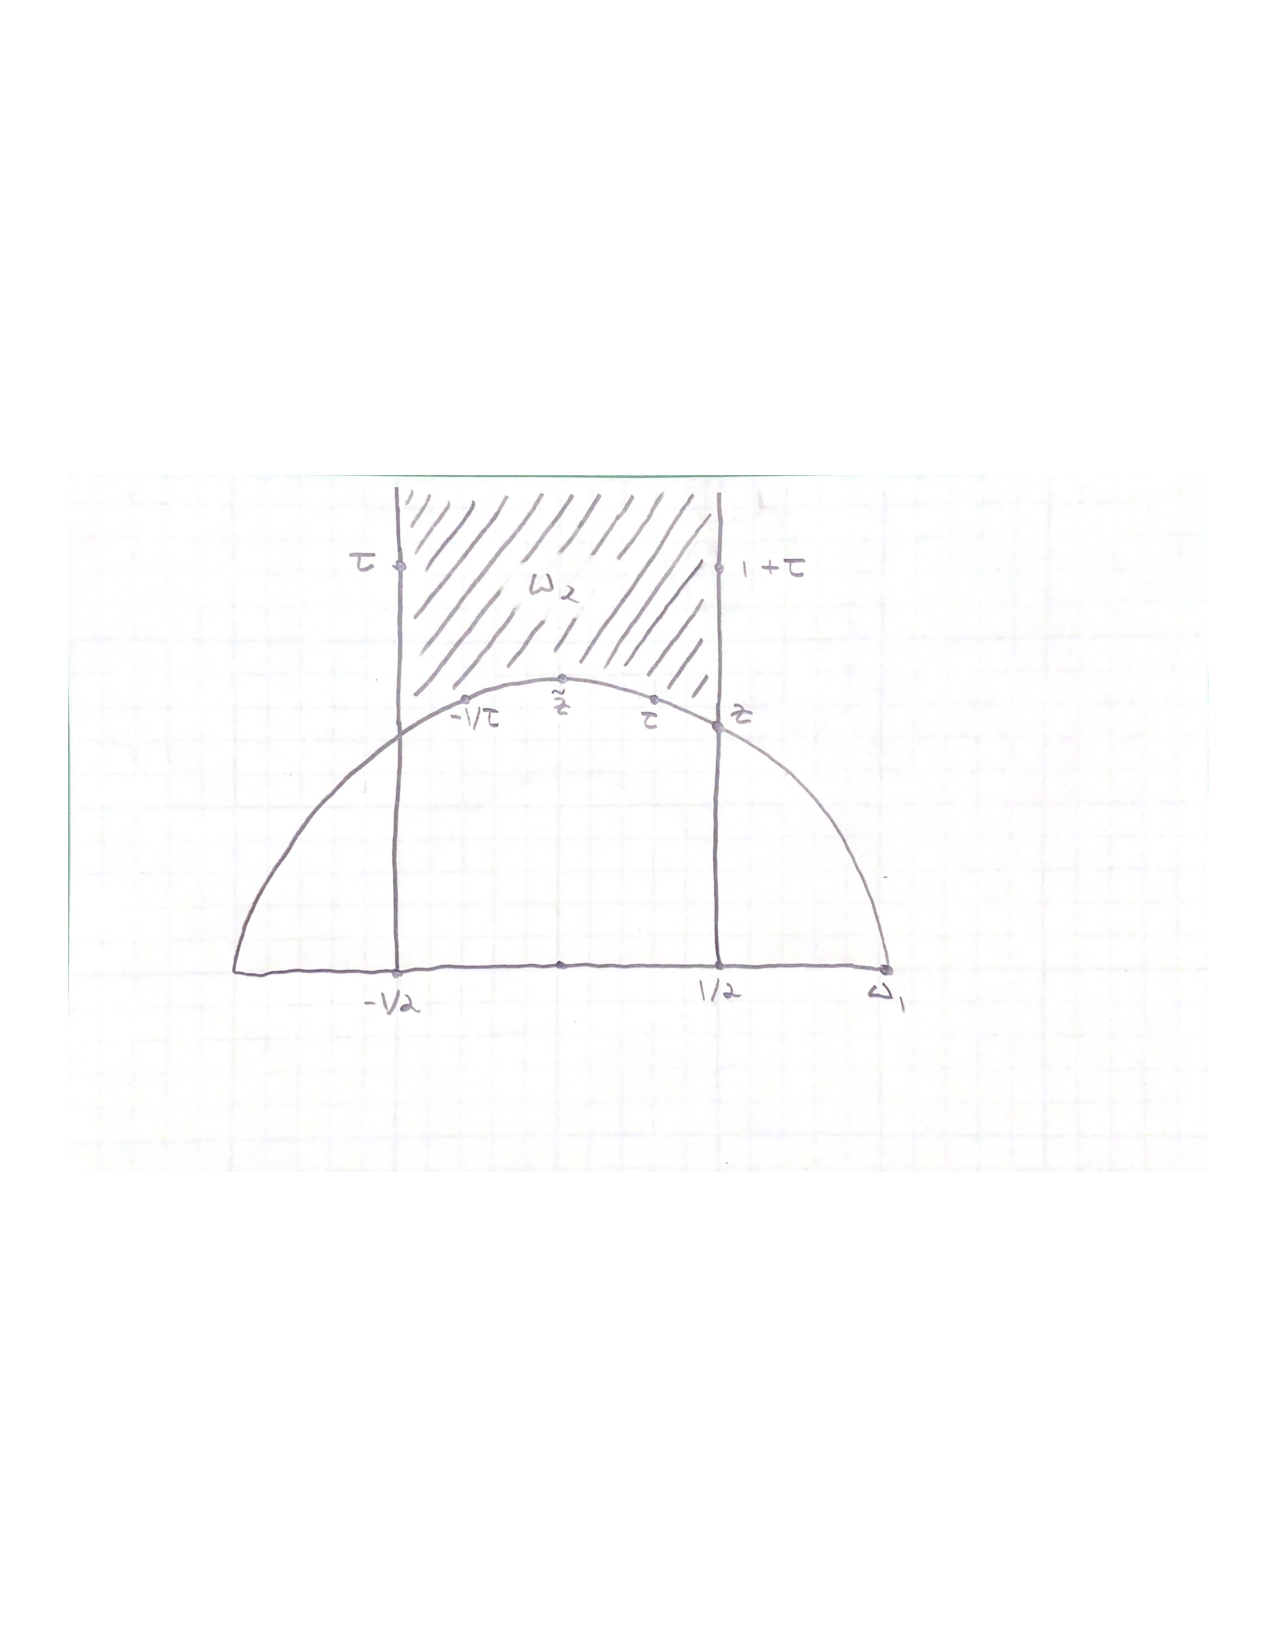
\includegraphics[scale=0.55]{fundamental_domain}
		\caption{The fundamental region of $\SL_{2}(\Z)$.}
	\end{center}
\end{figure}

We identify the points on the lines $\pm 1/2$ with each other, so imagine joining these two boundaries to create a sort of ``cylinder,'' and then close off the edges on the semicircle to close down one end of the ``cylinder.'' What results is something homeomorphic to an open disk. We want to make this disk into a sphere by adding in a point at infinity. 

If $f$ is a modular form, then $f(\tau) = f (\tau+1)$. Therefore,
\begin{align*}
	f(\tau) =  \sum_{n}^{}a_nq^n,\ q = \exp(2\pi i \tau). 
\end{align*}
This is expanded around $q=0$, so $\tau = i\infty$. The order of the root of $f$ at $i\infty$ is defined to be the order of the root of $\sum_{n}^{} a_nq^n$ at $q = 0$ (we will see why next lecture). If $f$ is holomorphic at $i\infty$, then $f(\tau) = a_0 + a_1q + \cdots$. The point $i\infty$ is called a \defn{cusp}\index{cusp} because, under $\tau \longmapsto -1/\tau$, this point is a cusp with respect to the fundamental region.

\begin{remark}
	The group $\SL_{2}(\Z)$ (or $\PSL_{2}(\Z)$) is an example of a {Fuchsian group}: a discrete subgroup of $\SL_{2}(\R)$ that acts on the upper-half plane. Another Fuchsian group is $\Gamma(N)$, given by this exact sequence:
	\begin{align*}
		\Gamma(N)  \longrightarrow \SL_{2}(\Z)  \longrightarrow \SL_{2}(\Z/N\Z)  \longrightarrow 1.
	\end{align*}
	The fundamental domain of $\Gamma(N)$ might be similar to that of $\SL_{2}(\Z)$, just with more cusps.

	Kleinian groups are discrete subgroups of $\SL_{2}(\C)$ acting on the Riemann sphere.
\end{remark}

\begin{figure}
	\begin{center}
		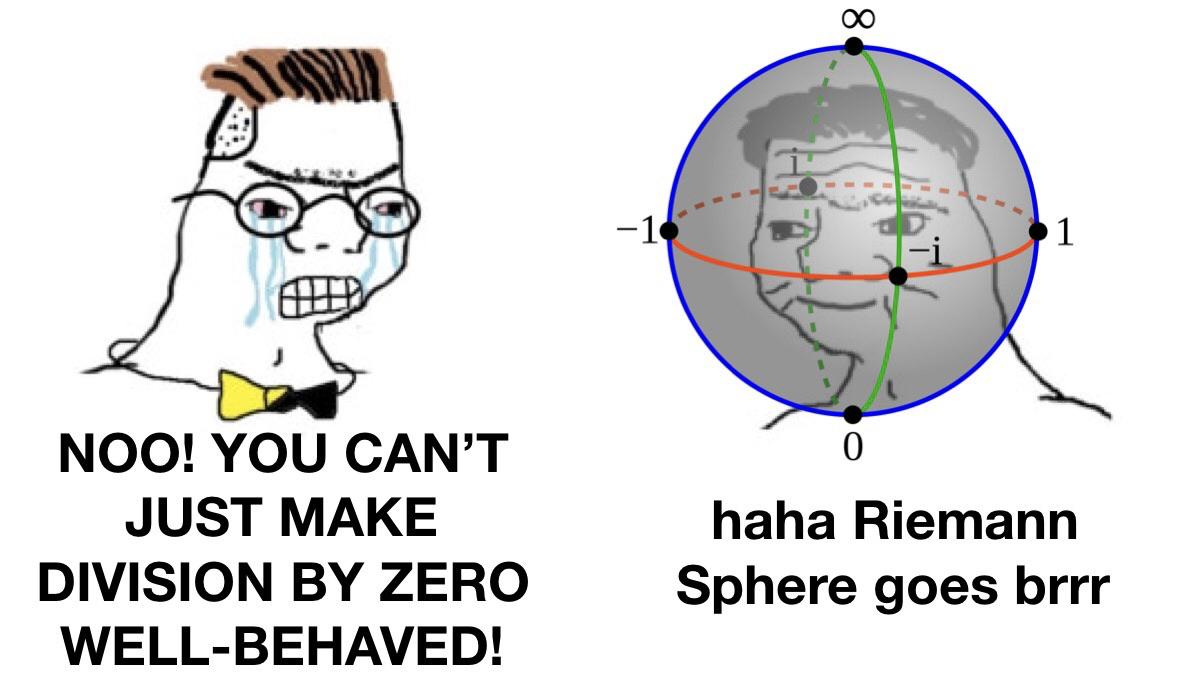
\includegraphics[scale=0.3]{riemann_sphere}
		\caption{A meme.}
	\end{center}
\end{figure}

\section{Classification}
Every modular form can be written as a polynomial in $E_4$ and $E_6$. 
\begin{lemma}[ ]\label{}\text{}
The number of roots of a weight-$k$ modular form in the fundamental domain of $\SL_{2}(\Z)$ is $k/12$.
\end{lemma}
\iffalse
How do we count roots, though? Recall that, if $f$ is holomorphic, 
\begin{align*}
	\#\textrm{roots} = \frac{1}{2\pi i}\int_{C}^{} \frac{f'(\tau)}{f(\tau)}  \, d\tau = \frac{1}{2\pi i} \int_{C}^{} \frac{df}{f}. 
\end{align*}

Suppose all roots of $f$ have imaginary part less than $t$. We cannot integrate around the fundamental domain, so we integrate up the line $\Re(t) = 1/2$ to the point $1/2 + it$, and then to $-1/2 + it$, then down to the unit semicircle, and then around the semicircle. Since $f(\tau) = f (\tau + 1)$, the integrals on the vertical lines cancel out. The integral along the horizontal line is $-1$ times the number of roots of $f$ at $\tau = i\infty$.

Okay: now we need to find the integral along the semicircle (from $\omega$ a cube root of unity to $\omega + 1$). Since 
 \begin{align*}
	f(-1/\tau) = \tau^k f (\tau).
\end{align*}
\fi
We have to count roots at $i\infty$, and we count fractional roots on the boundary. The number $1/12$ is the area of the fundamental domain divided by $4\pi$ (in hyperbolic space\iffalse, given by $dx\,dy/y^2$\fi). You can replace $\SL_{2}(\Z)$ with other groups and this still holds.

Now, let's classify modular forms that are holomorphic and on $\SL_{2}(\Z)$. Weight-$0$ forms have no roots given by the constants, so the dimension of this space is $1$. Forms of weight $2$ must have $1/6$ roots. Indeed, a root can have order $1/6$ at $\omega$ a cube root of unity. However, if there is a root at $\omega$, there is also one at $\omega + 1$ of weight $1/6$, such that the total number of roots is at least $1/3$. So there cannot be any modular forms of weight $2$.

Modular forms of weight $4$ must have $1/3$ roots, and the only way of getting this is to have roots at $\omega$ and $\omega + 1$. The space of forms of weight $4$ has dimension $1$: the roots of any modular form of weight $4$ are at $\omega$ and $\omega + 1$, so the quotient of two would be a modular form of weight $0$, which is a constant. That is, every modular form of weight $4$ is a scalar multiple of $E_4$.

Modular forms of weight $6$ must have $1/2$ roots. Indeed, one can get a root of order $1/2$ on the vertical boundary of the fundamental domain, but one also must have a root of order $1/2$ on the other side of the boundary. The only other option is to have a root at $i$. Therefore, $E_6$ has a root at $i$, and, similar to modular forms of weight $4$, all modular forms of weight $6$ are a scalar multiple of $E_6$. 

A modular form of weight $8$ must have $2/3$ roots, so it must have a ``double root'' (a root of order $1/3$) at $\omega$, and, hence, at $\omega + 1$. The modular form $E_4^2$ satisfies this, so, in fact, $E_4^2 = E_8$. As before, every modular form of weight $8$ is a scalar multiple of $E_8$. Modular forms of weight $10$ must have $5/6$ roots, and the only way to get this is to have a root at $i$, $\omega$, and $\omega + 1$. Therefore, we see that $E_{10} = E_4E_6$, and every modular form of weight $10$ is a scalar multiple of $E_{10}$.

Weight-$12$ modular forms must have $1$ root. One can think of three modular forms of weight $12$: $E_4^3$, $E_6^2$, and $E_{12}$. These all have the same constant term, but their $q$-expansions show that they are different. Let's consider the discriminant form:
\begin{align*}
	\Delta = \frac{E_4^3 -E_6^2 }{1728}.
\end{align*}
The form $\Delta$ vanishes at $i\infty$ since the constant terms cancel. The number $1728$ is the biggest number we can divide by to keep the coefficients integral. It is called the ``discriminant'' because it is related to the discriminant of an elliptic curve. Since the modular form $\Delta$ of weight $12$ has a root at $i\infty$, it is nonzero on the upper-half plane. 

Let $f$ be a modular form of weight $12$. Subtract a multiple of $E_4^3$ to make it vanish at $i\infty$. Then divide by $\Delta$. This is a holomorphic modular form of weight $0$, so it is a constant. Therefore, the space of modular forms of weight $12$ is two-dimensional. One sees that
\begin{align*}
	E_{12} = \frac{441}{691}E_4^3 + \frac{250}{691}E_6^2.
\end{align*}

For modular forms of even weight $k>12$, we repeat this process: that is, we take the modular form $E_4^\alpha E_6^\beta$ of weight $k$, take any modular form of weight $k$, subtract a multiple of $E_4^\alpha E_6^\beta$ to make it $0$ at $i\infty$, and divide by $\Delta$ to get a modular form of weight $k-12$. By induction, any modular form can be written as a polynomial in $E_4$ and $E_6$. So the ring of modular forms is the graded ring $\C[E_4,E_6]$.

\begin{exercise}\label{}\text{}
Show that $E_4$ and $E_6$ are algebraically independent. Hint: $E_4=0$ at $\omega$ but not at $i$, and $E_6=0$ at $i$ but not at $\omega$.
\end{exercise}

\section{Modular functions}
\begin{problem}
	Find all meromorphic (on $\H$ and at $i\infty$) modular functions. 
\end{problem}

Recall that
\begin{align*}
	j(\tau) =  \frac{E_4(\tau)^3}{\Delta(\tau)}.
\end{align*}
The modular function $j$ is holomorphic on $\H$ and has a pole of order $1$ at $i\infty$. It has a root of order $3$ at $\omega$. Further, $j(\tau)-1728$ has a root of order $2$ at $i$, since $E_6(\tau)$ has a root of order $1$ at $i$. We have already seen its Fourier expansion:
\begin{align*}
	j(\tau) = q ^{-1} + 744 + 196884q + \cdots.
\end{align*}

\begin{proposition}[ ]\label{}\text{}
Every modular function is a rational function in $j(\tau)$.
\end{proposition}

Suppose $f$ is a meromorphic modular function. First, we get rid of its poles by multiplying by $j(\tau)- j (\tau_0)$ which has a root at $\tau=\tau_0$. Further, $f$ is holomorphic on $\H$, but it might have a pole at $i\infty$. Write 
\begin{align*}
	f(\tau) = a_{-n}q^{-n} +\cdots.
\end{align*}
Then, we take
\begin{align*}
	f(\tau) - a_{-n} j (\tau) ^n = \alpha q^{1-n} + \cdots
\end{align*}
and repeat until $f$ has a root at $i\infty$. Then $f=0$. So, if $f$ is holomorphic on $\H$, then it is a polynomial in $j(\tau)$. 

In particular, this shows that $j$ is the simplest modular function. 
\begin{remark}
	It is very weird that the number $196884$ is hidden in the functional equation
	\begin{align*}
		f(\tau) = f (1 + \tau) = f  \left( - \frac{1}{\tau} \right).
	\end{align*}
\end{remark}

\begin{theorem}[Picard]\label{}\index{}\text{}
Suppose $f$ is a non-constant holomorphic function on $\C$. Then $f$ can miss out one complex number. That is, $f(\C) = \C$ or $f(\C)= \C \setminus  \{z\}$.
\end{theorem}

\begin{proof}
The derivative of $j(\tau)$ is a modular form of weight $2$ (it isn't holomorphic at $i\infty$, though). Therefore, the number of roots in the fundamental domain is $1/6$. We take a pole of order $m$ to be a root of order $-m$. By considering $j$, one can see that its derivative has a pole of order $1$ at $i\infty$. Further, it has roots of order $2$ at $\omega$ and $\omega + 1$ and a root of order $1$ at $i$. Altogether, we have
\begin{align*}
	-1 + 1/3 + 1/3 + 1/2 = 1/6
\end{align*}
roots.

Now, let's consider the multivalued inverse of $j$:
\begin{align*}
	j^{-1} : \C \longrightarrow \H.
\end{align*}
It has branch points at $j(\tau)$ when $j'(\tau) = 0$: that is, $\tau = \omega,i$, or their conjugates under $\SL_{2}(\Z)$. Therefore, $j^{-1}$ has branch points at $0$ and $1728$. 

Let $f:\C\longrightarrow \C$ be a holomorphic function. Suppose that $f(z) \ne 0,1728$ for all $z$. Then $j^{-1}(f(z)):\C\longrightarrow \H$ is holomorphic. Since $\left\lvert \exp(ij^{-1}(f(z))) \right\rvert <1$, $\exp(i j^{-1}(f(z)))$ is constant.
\end{proof}


\section{Discriminant and $E_2$}
Recall:
\begin{align*}
	\Delta = \frac{E_4^3 - E_6^2}{1728}.
\end{align*}
Further, $\Delta$ is nonzero on the upper-half plane. We will show that 
\begin{align*}
	\Delta(\tau) = q \prod  (1-q^n)^{24}.
\end{align*}

Formally,
\begin{align*}
E_2(\tau) = 1 - 24 \sum \sigma_1(n)q^n.	
\end{align*}
Further,
\begin{align*}
	\log \Delta (\tau ) = \log q - 24  \sum_{m,n}^{} \frac{q^{mn}}{m}.
\end{align*}
Differentiating, we get
\begin{align*}
	2\pi i - 2\pi i \cdot 24 \sum_{}^{} \sigma_1(n) q^n = 2\pi iE_2(\tau).
\end{align*}
That is,
\begin{align*}
	\frac{\Delta'(\tau)}{\Delta (\tau)} = 2\pi i E_2(\tau).
\end{align*}

Since $\Delta$ is a modular form,
\begin{align*}
	\Delta \left( -\frac{1}{\tau} \right) = \tau^{12} \Delta(\tau). 
\end{align*}
Therefore,
\begin{align*}
	E_2 \left( -\frac{1}{\tau} \right) = \tau^2  E_2(\tau) +  \frac{6\tau}{\pi i}.
\end{align*}
Notice the similarity with the following relation:
\begin{align*}
	\frac{1}{\Im(-1/\tau)} = \frac{1}{\Im(\tau)}\tau^2 - 2i\tau.
\end{align*}
Hence, we find that
\begin{align*}
	E_2(\tau) -  \frac{3}{\pi \Im(\tau)}
\end{align*}
is a modular form of weight $2$. However, the second term is not holomorphic.

Why isn't $E_2$ a modular form? Well, when we showed that $E_k$ was modular for $k\ge 4$, we required the absolute convergence of 
\begin{align*}
	\sum_{}^{} \frac{1}{(m+n\tau)^k},
\end{align*}
which is not absolutely convergent for $k=2$. However, it is absolutely convergent for $k= 2+\varepsilon$. Let's see if we can get something out of that.

The functional equation of $E_2$ is equivalent to that $\Delta$ is a modular form. Let's consider the Dedekind eta function:
\begin{align*}
	\eta(\tau) &:= q^{1/24} \prod  (1-q^n); \\
	\eta^{24}(\tau)&\phantom{:} = \Delta.
\end{align*}
This function satisfies
\begin{align*}
	\eta\left( -\frac{1}{\tau} \right) = \sqrt{\frac{\tau}{i}} \eta (\tau). 
\end{align*}
To prove this, we want to prove that
\begin{align*}
	\log \eta \left( \frac{i}{y} \right) - \log \eta \left( iy \right) = \frac{1}{2}\log y.
\end{align*}
Expanding, we want to prove that
\begin{align*}
	\sum_{m\ge 1}^{} \frac{1}{m(1-\exp(2\pi my))} = \sum_{m\ge 1}^{} \frac{1}{m(1-\exp(2\pi m/y))} + \frac{\pi}{12} \left(y - \frac{1}{y} \right) - \frac{\log y}{2}.
\end{align*}

Recall that $\pi/(\tan \pi z)$ has order-one poles at $\Z$. So $\sum_{}^{} f(n)$ has something to do with 
\begin{align*}
	\frac{1}{2\pi i} \int_{C}^{} f(z) \frac{\pi}{\tan \pi z} \, dz. 
\end{align*}
Consider 
\begin{align*}
	g(z) =  \frac{1}{z(\tan \pi i z) (\tan \pi z/y)}.
\end{align*}
The sum of the residues on the real axis corresponds to $\alpha_1\log \eta(iy) + \beta$. The sum of the residues on the imaginary axis corresponds to the terms of $\alpha_2 \log \eta(i/y) - \beta$. The residue at zero corresponds to $\alpha_3(y - 1/y)$. Further, as the contour's radius increases, the integral does not tend to $0$. What do we do?

Well, $(\tan \pi i z)(\tan \pi z/y)$ is approximately $+1$ in the top-left and bottom-right quadrants and approximately $-1$ in the top-right and bottom-left quadrants, so the integral of $g$ is approximately the integral of $z^{-1} \pm 1$, and what you get is $\alpha_4\log y$ as the radius of the contour tends to infinity.

So that ``proves'' that functional equation.

\begin{exercise}\label{}\text{}
Compute $\alpha_1,\beta,\alpha_2,\alpha_3,$ and $\alpha_4$.
\end{exercise}

\section{Theta functions}

An example of a theta function is
\begin{align*}
	\vartheta (\tau,z) := \sum_{n\in\Z}^{} e^{\pi i(n^2\tau + 2nz)}.
\end{align*}
The case \iffalse\textsl{Thetanullwerte}\fi in which $z=0$, which we will write $\vartheta (\tau)$, is a modular form in $\tau$. If one fixes $\tau$, $\vartheta(z)$ is almost elliptic. Finally, functions $\vartheta(\tau, z)$ are called \defn{Jacobi forms}\index{Jacobi form}. 

Clearly,
\begin{align*}
	\vartheta(\tau) =  \sum_{n}^{} e^{\pi i n^2\tau}
\end{align*}
is invariant under $\tau \longmapsto \tau + 2$. Further,
\begin{align*}
	\vartheta \left( -\frac{1}{\tau} \right) = \sqrt{\frac{\tau}{i}} \vartheta(\tau).
\end{align*}
Recall the Poisson summation formula where $\Lambda = \Z$:
\begin{align*}
	\sum_{n\in\Z}^{} f(n) &=  \sum_{n\in\Z}^{} \widehat{f}(n).
\end{align*}
Recall:
\begin{align*}
\widehat{f}(y) =  \int_{-\infty}^{\infty} e^{2\pi i x y} f(x) \, dx. 	
\end{align*}
If one writes $f(x) = e^{\pi x^2 i \tau}$, then $\widehat{f}(y) =  \sqrt{i/\tau} e^{\pi y^2/i\tau}$, and the functional equation follows.

But $\vartheta$ does not seem to be a modular form. Well, its two functional equations correspond to the matrices 
\begin{align*}
&	\mat{1&2\\0&1}; \\&\mat{0 &-1\\1&0}.
\end{align*}
These do not generate $\SL_{2}(\Z)$. However, conjugating the first by the second gives 
\begin{align*}
	\mat{1&0\\2&1}.
\end{align*}
This matrix and the first one generate 
\begin{align*}
	\Gamma(2) =  \left\{ \mat{a&b\\c&d} \equiv \mat{1&0\\0&1} \bmod 2 \right\} .
\end{align*}
Further, $\Gamma/\Gamma(2) \isomto  \SL_{2}(\F_2)$ has order $6$. The group
\begin{align*}
	\Gamma(2) \cup \mat{0&-1\\1&0} \Gamma (2)
\end{align*}
has index $3$ in $\SL_{2}(\Z)$. Therefore, $\vartheta$ is not modular over $\SL_{2}(\Z)$, but it is over a subgroup of $\SL_{2}(\Z)$ of index $3$.

\begin{remark}
	The function $\vartheta$ is a modular form with an eighth root of unity thrown in, which is almost as good.
\end{remark}
Now, as usual, write
\begin{align*}
	\zeta^*(s) := \Gamma \left( \frac{s}{2} \right) \pi^{-s/2}\zeta(s).
\end{align*}
This satisfies the functional equation
\begin{align*}
	\zeta^*(s) = \zeta^*(1-s).
\end{align*}
It turns out that one can show this by using the functional equation of $\vartheta$. Consider
\begin{align*}
	\frac{1}{2}\int_{0}^{\infty} \vartheta(ix) x^{s/2-1}  \, dx. 
\end{align*}
There's a problem, though: This integral does not converge for any $s$. For now, let's pretend it does converge and address that later. If it did, then it would be equal to $\zeta^*(s)$ by a straightforward change of variable. The result follows by the functional equation of $\vartheta$.

Now, suppose $x$ is large, and consider that integral again. We know that $\vartheta(ix)\approx 1$, so that integral is approximately
\begin{align*}
	\int_{1}^{\infty} x^{s/2-1}\, dx,
\end{align*}
which converges for $\Re(s)<0$ to $-2/s$, which can be continued to all $s\ne 0$. Similarly, suppose $x\approx 0$. Then $\vartheta(ix)\approx x^{-1/2}$. So that integral is approximately
\begin{align*}
	\int_{0}^{1} x^{-1/2} x^{s/2-1}  \, dx, 
\end{align*}
which converges for $\Re (s) > 1$ to $2/(s-1)$, which can be continued to all $s\ne 1$. However, since there are no numbers with real part less than $0$ and greater than $1$, this converges nowhere. 

We need to regularize it, then. Near $\infty$, we ``chop off'' the part of $\vartheta$ equal to $1$ and use the analytic continuation of the integral of $x^{s/2 -1}$. We do the same thing near $0$: We ``chop off'' the $x^{-1/2}$ from $\vartheta$ and deal with it separately.

Consider 
\begin{align*}
	\int_{}^{} x^{s-1}f(x)  \, dx. 
\end{align*}
Suppose, near $0$, 
\begin{align*}
	f(x) \sim \sum_{}^{} a_\lambda x^{-\lambda}
\end{align*}
and, near $\infty$, 
\begin{align*}
	f(x) \sim  \sum_{}^{} b_\mu x^{-\mu}.
\end{align*}
Again, we can regularize the integral by ``chopping off'' the $x^{-\lambda}$s that cause $f$ to diverge near $0$ and dealing with them separately. For each $a_\lambda x^{-\lambda}$, we get something with a pole at $s=\lambda$ or $s=\mu$. Therefore, $\zeta^*(s)$ has two poles at $s=0$ and $s=1$, which come from the fact that $\vartheta (ix)\approx 1$ for $x$ large and $\vartheta(ix) = x^{-1/2} $ for $x\approx 0$.
\section{Theta functions in higher dimensions}
Recall that
\begin{align*}
	\vartheta(\tau) =  \sum_{m\in\Z}^{} e^{\pi i m^2\tau}.
\end{align*}
Now, the idea is to replace $\Z$ with a lattice $\Lambda\subset \R^n$. Hence, we define
\begin{align*}
	\vartheta_\Lambda(\tau) :=  \sum_{\lambda\in \Lambda}^{} e^{\pi i\tau (\lambda,\lambda)}.
\end{align*}
Clearly,
\begin{align*}
	\vartheta_\Lambda(\tau + 2) = \vartheta_\Lambda (\tau)
\end{align*}
provided $(\lambda,\lambda) \in \Z$. Therefore, $\vartheta_\Lambda (\tau + 1) = \vartheta_\Lambda (\tau)$ provided $(\lambda,\lambda)\in 2\Z$.

Again, let's use the Poisson summation formula: 
\begin{align*}
	\sum_{\lambda\in \Lambda}^{} f(\lambda) =  \frac{1}{\left\lvert \Lambda \right\rvert }\sum_{\lambda\in \Lambda^* }^{} \widehat{f}(\lambda).
\end{align*}
Recall that the dual lattice $\Lambda^*$ is the set of all $\lambda\in \Lambda$ such that the inner product of $\lambda$ with everything else is an integer. Now, applying this to $f(\lambda) = e^{i\pi  (\lambda,\lambda) \tau}$, we find that
\begin{align*}
	\vartheta_{\Lambda} \left( -\frac{1}{\tau} \right) = \left( \frac{\tau}{i} \right) ^{n/2} \frac{1}{\left\lvert \Lambda \right\rvert } \vartheta_{\Lambda^*}(\tau).
\end{align*}
Suppose that $\Lambda =\Lambda^*$ and $\Lambda $ is even, so $(\lambda,\lambda)\in 2\Z$. Then
\begin{align*}
	\vartheta_{\Lambda } (\tau + 1) &= \vartheta_{\Lambda } (\tau);\\
	\vartheta_{\Lambda } \left( -\frac{1}{\tau} \right) &= \left( \frac{\tau}{i} \right) ^{n/2}\vartheta_{\Lambda }(\tau).
\end{align*}
These are transformations under all of $\SL_{2}(\Z)$.

Consider the $E_8$ lattice: Take all vectors $(n_1,\hdots, n_8)$ where $\sum_{i}^{} n_i$ is even and either all $n_i\in \Z$ or all $n_i\in \Z+1/2$. Indeed, this lattice is even and self-dual. This works provided $8$ divides the dimension. (This lattice is the root lattice of the $E_8$ Lie algebra.) Therefore, we get
\begin{align*}
	\vartheta_{E_8 }(\tau + 1) &= \vartheta_{E_8 }(\tau) ;\\
	\vartheta_{E_8 } \left( -\frac{1}{\tau} \right) &= \left( \frac{\tau}{i} \right) ^{8/2} \vartheta_{E_8 }(\tau)\\
							&= \tau^{4} \vartheta_{E_8 } (\tau).
\end{align*}
Therefore, $\vartheta_{E_8 }$ is a modular form of level one and weight $4$, so
\begin{align*}
	\vartheta_{E_8 } (\tau) &=  E_4(\tau) \\
				&= 1 +240 \sum_{n}^{} \sigma_3(n)q^n\\
				&= 1 + 240q + 2160q^2 + \cdots.
\end{align*}
(Man, that notation is unfortunate.)  Let's check this explicitly.

Let's consider the vectors with norm $2$: Vectors of the form $(0,\hdots, \pm 1,\hdots,\pm 1,\hdots,0)$ have norm $2$, and there are $112$ of them. Vectors of the form $(\pm 1/2,\hdots,\pm 1/2)$ also have norm $2$, and there are $128$ of these. Indeed, in total, we get $240$ vectors of norm $2$. The dimension of $E_8$ Lie algebra is $240 + 8$, that is, the number of norm-$2$ vectors plus the dimension of $E_8$.) 

Now, vectors of norm $4$: Vectors $(0,\hdots,\pm 1,\hdots,\pm 1,\hdots, \pm_1,\hdots,\pm 1,\hdots, 0)$ have norm $4$, and there are $1120$ of these. Vectors $(\pm 3/2,\pm 1/2,\hdots, \pm 1/2)$ also have norm $4$, and there are $1024$ of these. Lastly, vectors of the form  $(0,\hdots, \pm 2,\hdots, 0)$ have norm $4$, and there are $16$ of them. Altogether, we have $2160$ vectors.

\begin{problem}
	Can you hear the shape of a drum?
\end{problem}

Take a Riemannian manifold $M$ and consider the eigenvalues of the Laplace operator on it. We take $M=\R^n/\Lambda$, and the eigenvalues of the Laplacian correspond to the norms of vectors in $\Lambda$. Are there two lattices with the same number of vectors with any given norm---the same theta function? Milnor pointed out that $E_8^2$ and $E_{16}$ satisfy this. Both of their theta functions are modular forms of weight $8$, and the space of modular forms of weight $8$ is $1$-dimensional, so that theta function must be the Eisenstein series $E_8(\tau)$. These lattices are distinct, for $E_8^2$ can be split into $2$ nonempty orthogonal subsets and $E_{16}$ cannot. That is, these lattices generate different Riemannian manifolds but have the same spectrum, ``so if you had these $16$-dimensional drums, they would sound exactly the same.''

\begin{problem}
	How many length-$\sqrt{4} $ vectors are there in the Leech lattice?
\end{problem}

Well, the Leech lattice is even, unimodular (that is, self-dual), $24$-dimensional, and has no vectors of length $\sqrt{2} $. The corresponding theta function is a modular form of weight $12$, and the space of modular forms is $2$-dimensional and spanned by $E_4^3$ and $\Delta$. The coefficient of $q^0$ must be $1$ since there's only one vector of norm $0$. The coefficient of $q^1$ must be $0$ since there are no vectors of norm $\sqrt{2} $. Therefore,
\begin{align*}
	\vartheta _{II_{25,1}} &= E_4^3 - 720\Delta\\
			       &= 1 + 0q + 196560q^2 + \cdots.
\end{align*}

\begin{exercise}\label{}\text{}
Do the same thing in $32$ dimensions. There are more than $10000000$ unimodular, even lattices with no vectors of norm $\sqrt{2} $, as Oliver King proved\footnote{``A mass formula for unimodular lattices with no roots,'' 2002.}.
\end{exercise}

\begin{problem}
	Can we find an even, unimodular lattice with positive dimension less than $8$?
\end{problem}

No: The dimension must be divisible by $8$. Suppose not, and let $\Lambda$ be such a lattice. Then we can repeatedly take direct sums of $\Lambda$ such that the resulting dimension of the lattice is congruent to $4$ mod $8$. Therefore, we can show that a lattice of dimension $4$ mod $8$ cannot satisfying these properties cannot be. The lattice $\Lambda$ would satisfy
\begin{align*}
	\vartheta_{\Lambda } \left( \frac{a\tau + b}{c\tau + d} \right) &= \chi \mat{a&b\\c&d} (c\tau + d)^{n/2} \vartheta_{\Lambda } (\tau)
\end{align*}
where $\chi$ is a character, so $\chi(AB) = \chi (A)\chi  (B)$. Further, we must have
\begin{align*}
	\chi \mat{1&1\\0&1} &= \chi(T) = +1;\\
	\chi\mat{0&-1\\1&0} &=\chi(S) = -1.
\end{align*}
However, $(ST)^3 = 1$ in $\PSL_{2}(\Z)$. So $\chi(ST)^3 =+1$, which contradicts that $\chi(T)=+1$ and $\chi(T)=-1$. The result follows. 


\section{Hecke operators}
Suppose
\begin{align*}
	f\left( \frac{a\tau + b}{c\tau + d} \right) = f(\tau)
\end{align*}
where
\begin{align*}
	\mat{a&b\\c&d} \in \SL_{2}(\mathbf{Z}).
\end{align*}
The function $f(2\tau)$ is invariant under the matrix
\begin{align*}
	\mat{a&b/2\\2c&d}.
\end{align*}
Now,
\begin{align*}
	\left\{ \mat{a&b/2\\2c&d} : a,b,c,d\in \mathbf{Z} \right\} \cap \SL_{2}(\mathbf{Z}) = \left\{ \mat{a&b\\2c&d} : a,b,c,d\in \mathbf{Z} \right\} 
\end{align*}
is a group notated $\Gamma_0(2)$ of index $3$ in $\SL_{2}(\Z)$ under which $f(2\tau)$ is invariant. We can make it invariant under $\SL_{2}(\Z)$ by summing over $3$ cosets, which gives
\begin{align*}
	f(2\tau) + f \left( \frac{\tau}{2} \right) + f\left( \frac{\tau+1}{2} \right) .
\end{align*}
The action of $\tau \longmapsto \tau+1$ swaps the last two summands and takes the first to itself. The action of $\tau \longmapsto -1/\tau$ swaps the first two summands and takes the last to itself. This operator is sometimes notated $T_2(\tau)$. It is a Hecke operator.

\begin{example}[ ]\label{}\text{}
Let $f(\tau) := j (\tau) - 744$. So
\begin{align*}
	f(\tau) &= q ^{-1} + 196884 q + 21493760 q^2 + 864299970q^3 + 20245856256q^4 + \cdots\\
	&= q^{-1} + c_1q + c_2q^2 + c_3q^3 + c_4q^4 + \cdots.
\end{align*}
Now
\begin{align*}
	f(2\tau) &= q^{-2} +  c_1q^2 + c_2q^4 + \cdots;\\
	f \left( \frac{\tau}{2} \right) + f\left( \frac{\tau + 1}{2} \right) &= 2c_2q + 2c_4q^2 + 2c_6q^3 + \cdots .
\end{align*}
Therefore,
\begin{align*}
	f(2\tau) + f \left( \frac{\tau}{2} \right) + f\left( \frac{\tau + 1}{2} \right) &= q^{-2} + 2c_2q + \cdots\\
											&= f(\tau)^2 - 2\cdot 196884
\end{align*}
is a modular function. Comparing the $q^2$ coefficients, we find
\begin{align*}
	2c_3 + c_1^2 = 2c_4 + c_1.
\end{align*}
We can get more interesting identities by considering more terms or considering $f(n\tau)$.
\end{example}

Recall that we can think of $f$ as a function of lattices in $\mathbf{C}$, so $f(\tau)$ corresponds to a lattice $\langle 1,\tau\rangle$. Suppose $\Lambda \subset \C$ is a lattice. Then
\begin{align*}
	\sum_{\substack{\textrm{lattices }L\subset \Lambda\\\left\lvert \Lambda/L \right\rvert =2}}^{}f(L)
\end{align*}
is a function of lattices. There are three such sublattices: $\langle 2,\tau\rangle$, $\langle 2,\tau+1\rangle$, and $\langle 1,2\tau\rangle$. One can see that these correspond to $f(\tau/2)$, $f((\tau + 1)/2)$, and $f(2\tau)$ respectively. 

However, it's not exactly the same. Applying what we did before with $f(4\tau)$, we get
\begin{align*}
	f(4\tau) + f \left(\frac{2\tau + 1}{2} \right) + f\left( \frac{\tau}{4} \right) + f \left( \frac{\tau + 1}{4} \right) + f \left( \frac{\tau+2}{4} \right) + f\left( \frac{\tau+3}{4} \right) .
\end{align*}
If we sum over all lattices of index $4$, we get another term corresponding to
\begin{align*}
	f\left( \frac{2\tau + 0}{2} \right) = f(\tau).
\end{align*}
If we look at $f(n\tau)$ where a square divides $n$, we find a slight difference.

Performing row reduction, we find that 
\begin{align*}
	\left\{ \mat{2&0\\0&1},\mat{1&0\\0&2},\mat{1&1\\0&2} \right\} 
\end{align*}
are representatives of the left cosets of determinant-$2$ matrices mod determinant-$1$ matrices. These correspond to $2\tau$, $\tau/2$, and $(\tau+1)/2$ respectively. So, we sum
\begin{align*}
	\sum_{}^{} f\left( \frac{a\tau + b}{c\tau + d} \right) 
\end{align*}
and, again, we get a modular function. This is another way to get Hecke operators.

In general, we can replace $2$ with $n$, and we get a Hecke operator $T_n$. Let $M$ be the set of left cosets of matrices of determinant $n$ modulo matrices of determinant $1$. Performing row operations, one finds that these matrices are of the form 
\begin{align*}
	\mat{n/d & \alpha\\0&d}
\end{align*}
where $d$ is a divisor of $n$ and $\alpha \in \{0,1,\hdots, d-1\}$. We find that (abusing notation)
\begin{align*}
	\sum_{M}^{} j\left( \frac{a\tau + b}{c\tau + d} \right) = \sum_{}^{} j\left( \frac{n\tau/d + \alpha}{d} \right). 
\end{align*}
This reduces quite nicely when $n=p$ is prime. We get 
\begin{align*}
	f(p\tau) + f  \left( \frac{\tau}{p} \right) + f\left( \frac{\tau + 1}{p} \right) + \cdots + f \left( \frac{\tau + p - 1}{p} \right) .
\end{align*}
is a modular function. 

\section{Product formula for $j$}
Recall that
\begin{align*}
	j(\tau) - 744 &= q ^{-1} + 196884q + 21493760q^2 + \cdots\\
		      &= \sum_{}^{} c_nq^n.
\end{align*}
Last time, we showed how to find nonlinear relations between the $c_n$s, the simplest of which is
\begin{align*}
	2c_3 + c_1^2 = 2c_4 + c_1.
\end{align*}
One can understand these relations by the formula
\begin{align*}
	j(\sigma)-j(\tau) &= p^{-1} \prod_{\substack{ m > 0\\n\in \Z}} (1-p^mq^n)^{c_{mn}}
\end{align*}
where $p=\exp(2\pi i \sigma)$ and $q = \exp(2\pi i \tau)$. The right hand side does not seem antisymmetric in $p$ and $q$, but $p^{-1}(1-pq^{-1}) = (p^{-1}-q^{-1})$, and the other terms work out similarly.

The formula \begin{align*}
	j(\sigma)-j(\tau) &= p^{-1} \prod_{\substack{ m > 0\\n\in \Z}} (1-p^mq^n)^{c_{mn}}
\end{align*}
is very similar to the Weyl denominator formula for a finite-dimensional Lie algebra:
\begin{align*}
	\sum_{w\in W}^{} \epsilon(w)e^{w (-\rho)} &= e^{-\rho} \prod_{\alpha \textrm{ positive root}}  (1-e^\alpha)^{\mult \alpha} \\&= e^{-\rho} \prod_{\alpha \textrm{ positive root}}  (1-e^\alpha)
\end{align*}
where $W$ is the Weyl group, $\epsilon$ is $\pm 1$ (given by the determinant of the action of $w$ on the Cartan subalgebra), and $\rho $ is a Weyl vector. It turns out that the product formula for the elliptic modular function $j$ really is somewhat analgous to this: It is the denominator formula for the infinite-dimensional monster Lie algebra where the $c_{mn}$s are the multiplicities of the roots of the monster Lie algebra.

If we have a function $\sum_{}^{} c_nq^n$ and we apply the Hecke operator $T_m$ to it, what do we get? Well, we get
\begin{align*}
	\sum_{n}^{} q^n \sum_{k\, \mid \, (m,n)}^{} \frac{m}{k}c_{mn/k^2}.
\end{align*}
Secondly, a modular function that is holomorphic on $\H$ is determined by its coefficients of $q^0,q^{-1}, q^{-2}$, etc. (Recall that we showed that any modular function that is holomorphic at $i\infty$ and on $\H$ is constant.)

Now, let's apply $\log$ to that infinite product:
\begin{align*}
	\log \prod_{\substack{ m > 0\\n\in \Z}} (1-p^mq^n)^{c_{mn}} &= - \sum_{\substack{m>0\\n\in \Z}}^{} \sum_{k}^{} c_{mn} \frac{p^{ m k} q^{nk}}{k}\\
								    &= -\sum_{m>0}^{} p^m \sum_{n\in \Z}^{} \sum_{k\,\mid\,(m,n)}^{} \frac{1}{k} c_{mn/k^2}q^n\\
								    &= - \sum_{m}^{} p^m \frac{T_m}{m}(j(\tau)- 744).
\end{align*}
So, applying $\exp$,
\begin{align*}
	p^{-1} \prod_{\substack{ m > 0\\n\in \Z}} (1-p^mq^n)^{c_{mn}} = \sum_{m}^{} p^m \times \textrm{modular function in $\tau$}. 
\end{align*}
Doing some rough work with the coefficients\footnote{See \url{https://youtu.be/CBfDbJIaPJo?t=657}.}, the formula for $j$ follows.
\begin{figure}
	\begin{center}
		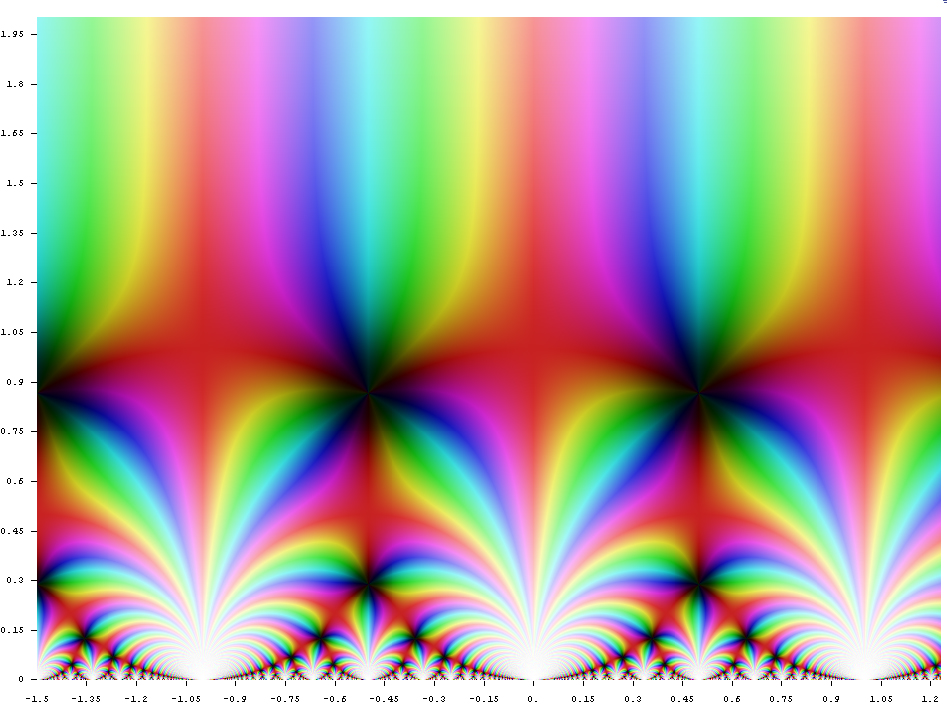
\includegraphics[scale = 0.4]{j}
                \caption{$j(\tau)$ on the upper-half plane.}
	\end{center}
\end{figure}

\section{Hecke operators for forms}

Recall how we got the Hecke operator $T_2$ of a modular function:
\begin{enumerate}
	\item We can make $f(2\tau)$ invariant under $\SL_{2}(\mathbf{Z})$ by taking
		\begin{align*}
			f(2\tau) + f \left( \frac{\tau}{2} \right) + f \left( \frac{\tau+1}{2} \right) ;
		\end{align*}
	\item We sum over lattices of index $2$ of $\langle 1,2\rangle $. There are three such lattices, and they correspond to the three terms above;
	\item The matrices 
		\begin{align*}
			\mat{2&0\\0&1}; \mat{1&0\\0&2} ;\mat{1&1\\0&2};
		\end{align*}
		correspond to these three terms.
\end{enumerate}
We do something very similar for modular forms of weight $k>0$. Instead of considering an invariant function $f$, we consider an invariant form $f(\tau)  (d\tau)^{ k/2}$, which just results in some extra constants in the final analysis. 

For instance, now, we have
\begin{align*}
&\phantom{=}\,\ \,	f(2\tau)  (d 2\tau)^{k/2} + f\left( \frac{\tau}{2} \right) \left( d \frac{\tau}{2} \right) ^{k/2} + f\left( \frac{\tau+1}{2} \right) \left( d \frac{\tau+1}{2} \right) ^{k/2}\\ &= \left[2^{k/2}f(2\tau) + 2^{-k/2}f \left( \frac{\tau}{2} \right) + 2^{-k/2}f \left( \frac{\tau+1}{2} \right) \right](d\tau)^{k/2}.
\end{align*}

We can do the same thing for any integer $n$. Suppose $f(\tau) :=  \sum^{} c(m)q^m$. Then
\begin{align*}
	T_n(f) &=  \sum_{}^{} f\left( \frac{a\tau+b}{d} \right)  
\end{align*}
where $ad = n$ and $0\le b< n$. (Recall that 
\begin{align*}
	\mat{a&b\\0&d}
\end{align*}
is a coset representative of determinant-$n$ matrices mod determinant-$1$ matrices.) One finds that the Fourier transformation of $T_n$ is
\begin{align*}
	T_n(f) =  \sum_{m}^{} q^m \sum_{d\,\mid\,(m,n)}^{}  d^{k-1} c \left( \frac{mn}{d^2} \right). 
\end{align*}
For example,
\begin{align*}
	T_2(f) =  c_0 + 2^{k-1} c_0 +c_2q + (c_4 + 2^{k-1}c_1)q^2 + \cdots. 
\end{align*}

Let us study this for the weight-$12$ cusp form 
\begin{align*}
	\Delta(\tau) = q \prod_{n>0}  (1-q^n)^{24}.
\end{align*}
Recall that the space of these is one-dimensional. Therefore, $\Delta$ is an eigenfunction of all $T_n$. Now
\begin{align*}
	\Delta (\tau) &= q - 24q^2+252q^3 - 1472q^4 + 4830q^5 - 6048q^6 + \cdots\\
		      &= \tau(1)q + \tau (2)q^2 + \tau (3)q^3 + \tau (4)q^4 + \tau (5)q^5 + \tau (6)q^6 + \cdots.
\end{align*}
Notice that $(-24)\cdot 252= -6048$. Why? First, note that
\begin{align*}
	T_n(\Delta) = \tau (n) q^1 + \cdots,
\end{align*}
so the eigenvalue of $T_n$ on $\Delta$ is $\tau(n)$ (the coefficient of $q^n$). Now, $T_mT_n = T_{mn}$ whenever $(m,n)=1$ since $T_m$ is a sum of lattices of index $m$, $T_n$ is a sum of lattices of index $n$, and if $L\supseteq M$ is such that $L/M$ is abelian of order $mn$ where $(m,n)=1$, $L/M$ has one subgroup of index $m$ and one of index $n$, so any sublattice of index $mn$ can be written uniquely by taking a sublattice of index $m$ and a sublattice of index $n$. Therefore, since the eigenvalue of $T_n$ is $\tau(n)$, $\tau(m)\tau (n)= \tau (mn)$ whenever $(m,n)$ is coprime.

What about other relationships between coefficients? Well,
\begin{align*}
	T_2(\Delta) = \tau (2)q +  (\tau(4)+ 2^{11}\tau (1)) q^2 + \tau(6)q^3 +  (\tau(8)+2^{11}\tau (2)) q^4 + \cdots,
\end{align*}
and
\begin{align*}
	\Delta(\tau) = \tau (1) q + \tau (2)q^2 + \tau (3)q^3 + \tau (4)q^4 +\cdots.
\end{align*}
We see that  $\tau(1)\tau(2) = \tau(2)$, and one can verify that $\tau(2)^2 = \tau (4) + 2^{11} \tau (1)$. Further,
\begin{align*}
	\tau(2) \tau (2^n) = \tau (2^{n+1}) +  2^{11}\tau (2^{n-1}),
\end{align*}
and, more generally,
\begin{align*}
	\tau(p)\tau (p^n) = \tau(p^{n+1}) + p^{11} \tau (p^{n-1}).
\end{align*}

We discovered some nonlinear relations between the coefficients of the elliptic modular function that applying Hecke operators to it. Here, we have the same thing. For the elliptic modular function, we encoded these relations in an infinite product:
\begin{align*}
	j(\sigma)-j(\tau) &= p^{-1} \prod_{\substack{ m > 0\\n\in \Z}} (1-p^mq^n)^{c_{mn}}.
\end{align*}
We can do the same for $\Delta$, but it looks much different. It turns out it's an Euler product.

Take the Mellin transform of $\Delta$:
\begin{align*}
	\int_{0}^{\infty} \Delta(it) t^{s-1} \, dt. 
\end{align*}
Since
\begin{align*}
	\int_{0}^{\infty} \exp({2\pi i n t})t^{s-1}  \, dt = (2\pi)^{-s}  \frac{\Gamma(s)}{n^s}, 
\end{align*}
we find that
\begin{align*}
	\int_{0}^{\infty} \Delta(it) t^{s-1} \, dt	&=(2\pi)^{-s} \Gamma (s)  \sum_{n}^{} \frac{\tau(n)}{n^s}.	
\end{align*}
Call that Dirichlet series $L(s)$, and call the above $L^*(s)$. Since
\begin{align*}
	\Delta \left( -\frac{1}{\tau} \right) &= \tau^{12}\Delta(\tau),
\end{align*}
one finds that
\begin{align*}
	L^*(12-s) = L^* (s).
\end{align*}
(There is a conjecture analgous to the Riemann hypothesis for $L^*$ where the nontrivial roots have real part $6$. The Mellin transform of $\Delta$ is nicer than that of the Riemann zeta function since $\Delta$ vanishes at the cusp, so the transform converges for all $s$ and $L$ does not have any poles.) Recall that
 \begin{align*}
	\zeta(s) = \prod_{p \textrm{ prime}}  \frac{1}{1-p^{-s}}.
\end{align*}
Notice:
\begin{align*}
	L(s) &=  \sum_{n}^{} \frac{\tau(n)}{n^s}\\
	     &= \prod_{p\textrm { prime}} \left( \frac{1}{p^0} + \frac{\tau(p)}{p^s}  + \frac{\tau(p^2)}{p^{2s}} + \cdots \right)\\
	     &= \prod_{p\textrm{ prime}} \frac{1}{1-\tau(p)p^{-s} + p^{11-2s}}.
\end{align*}

Ramanujan conjectured and Deligne proved\footnote{``Formes modulaires et repr\'esentations $\ell$-adiques,'' 1969 and ``La conjecture de Weil: I,'' 1974.} that the roots of 
\begin{align*}
	1 - \tau(p) z + p^{11} z^2
\end{align*}
are complex conjugate. This is equivalent to
\begin{align*}
	\left\lvert \tau(p) \right\rvert \le 2p^{11/2}.
\end{align*}
Also, this implies that
\begin{align*}
	\left\lvert \tau(n) \right\rvert \le n^{11/2}\sigma_0 (n)
\end{align*}

\begin{exercise}\label{}\text{}
The spaces of cusp forms of weight $12$, $16$, $18$, $20$, $22$, and $26$ is one-dimensional spanned by $\Delta$, $\Delta E_4$, $\Delta E_6$, $\Delta E_8$, $\Delta E_{10}$, and $\Delta E_{14}$. Find analogues for Ramanujan's work on $\Delta$.
\end{exercise}


\section{Petersson inner product}

Recall: If $f$ is an eigenfunction of the Hecke operators, then we get relations between the coefficients. What if the space of forms has dimension greater than $1$? We will show that it is spanned by eigenfunctions $T_n$. Recall that if $T_n$ commute and are self-adjoint, then the vector space $V$ on which they act has a basis of eigenforms. (Self-adjoint means that we need a sesquilinear form $(\cdot,\cdot)$ on the space of modular forms.)

Notice that $T_m$ and $T_n$ commute when $m$ and $n$ are coprime. We also showed that $T_pT_{p^n} = T_{p^{n+1}} + p^{2k-1}T_{p^{n-1}}$. So, the algebra of operators spanned by $T_p,T_{p^2},\hdots$ is generated by $T_p$. So all $T_n$ commute.

Now, what about self-adjointness? Well, what is the inner product? There is a measure $dx\,dx/y^2$ on $\H$ invariant under $\SL_{2}(\R)$. Therefore, if $f$ and $g$ are modular functions, it makes sense to define
\begin{align*}
	(f,g) =  \int_{\textrm{fundamental domain of $\SL_{2}(\Z)$}} fg\frac{dx\,dy}{y^2}. 
\end{align*}
However, this appears to diverge. For example, $jg$ will typically have a term of $q^{-n}$, and $\left\lvert q^{-n} \right\rvert = \exp(2\pi ny)$ gets huge.

We can regularize, though. It turns out that the integrals obtained by cutting off the fundamental domain at some horizontal line are the same\footnote{See \url{https://youtu.be/wWTMTSmOBL4?t=362}.}. Therefore, we can take
\begin{align*}
	(f,g) := \lim_{\varpi\to\infty}  \int_{\textrm{fundamental domain cut off at $\varpi$} }fg\frac{dx\,dy}{y^2}. 
\end{align*}
This is well-defined if $f$ and $g$ are holomorphic (on $\H$) modular functions. For example, we find that
\begin{align*}
	(j-720, 1) = 0.
\end{align*}
This is why $24$ is a much more natural constant term for $j$ than $744$.

We would like to do this for modular forms.
\begin{problem}
	Suppose $f$ and $g$ are modular forms of weight $k$. Then $fg$ and $f \overline{g}$ are not invariant under $\SL_{2}(\R)$, so the integral around the fundamental domain of $f \overline{g}$ with respect to the mentioned metric is not defined. It depends on the fundamental domain. How do we define an inner product?
\end{problem}

Notice that $f(\tau) (d\tau)^{k/2}$ is invariant under, and so is $\overline{g(\tau)} (d \overline{\tau}) ^{k/2}$. Well, 
\begin{align*}
	d  \left( -\frac{1}{\tau} \right) &= \frac{d\tau}{\tau^2};\\
	d \left( -\frac{1}{\overline{\tau}} \right) &= \frac{d \overline{\tau}}{\overline{\tau}^2};\\
	\Im \left( -\frac{1}{\tau} \right) &= \frac{\Im(\tau)}{\tau \overline{\tau}}. 
\end{align*}
Considering these equalities, one sees that 
\begin{align*}
	\frac{d\tau d \overline{\tau}}{\Im(\tau) ^2}
\end{align*}
is invariant under $\SL_{2}(\R)$. Therefore, if $f$ and $g$ have weight $k$, then
\begin{align*}
	f(\tau) \overline{g(\tau)} \Im(\tau)^k
\end{align*}
is invariant. Hence, one defines
\begin{align*}
	(f,g) :=  \int_{\textrm{fundamental domain}} f(\tau) \overline{g(\tau)} \Im(\tau)^k \frac{dx\,dy}{\Im(\tau)^2}. 
\end{align*}
One can check that the $T_n$ are Hermitian, so
\begin{align*}
	(T_n(f),g) =  (f, T_n(g)).
\end{align*}
Thus, the cusp forms have a basis of eigenforms of $T_n$. 

Anything one can do with $\Delta$ can be done with all of these eigenforms. Recall that
\begin{align*}
	\sum_{n}^{} \frac{\tau(n)}{n^s} = \prod_{p \textrm{ prime}} \frac{1}{1-\tau(n)p^{-s} + p^{11-2s}}.
\end{align*}
Suppose that $f = \sum c(n)q^n$ is a modular form of weight $k$. Then
\begin{align*}
	\sum_{n}^{} \frac{c(n)}{n^s} = \prod_{p\textrm{ prime}} \frac{1}{1 - c(n)p^{-s} + p^{k-1-2s}}
\end{align*}
Recall that Ramanujan conjectured that
\begin{align*}
	\left\lvert \tau(p) \right\rvert \le 2p^{11/2}.
\end{align*}
Petersson generalized this conjecture, to guess that
\begin{align*}
	\left\lvert c(p) \right\rvert \le 2p^{(k-1) /2}.
\end{align*}
Deligne proved both of these.

\begin{exercise}\label{}\text{}
Find the eigenforms of weight $24$, the first case when the space of cusp forms has dimension greater than $1$. (Warning: The answer is messy. The eigenforms do not have integer coefficients, but those defined over an imaginary quadratic field. In general, this is how eigenforms of heigher weight tend to look.)
\end{exercise}

\printindex
\end{document}
